% A skeleton file for producing Computer Engineering reports
% https://kgcoe-git.rit.edu/jgm6496/KGCOEReport_template

\documentclass[CMPE]{../KGCOEReport}

% The following should be changed to represent your personal information
\newcommand{\classCode}{EEEE 380}  % 4 char code with number
\newcommand{\name}{Andrei Tumbar}
\newcommand{\LabSectionNum}{1}
\newcommand{\LabInstructor}{Dr.\ Moon}
\newcommand{\TAs}{Karen Chen}
\newcommand{\exerciseNumber}{3}
\newcommand{\exerciseDescription}{CMOS Inverter Design and Dynamic Behavior}

\usepackage{tikz}
\usepackage{circuitikz}
\usepackage{multirow}
\usepackage{titlesec}
\usepackage{float}
\usepackage{lmodern}
\usepackage{siunitx}
\usepackage{subcaption}
\usepackage{graphicx}
\usepackage[usestackEOL]{stackengine}
\usepackage{scalerel}
\usepackage[T1]{fontenc}
\usepackage{amsmath}


\def\code#1{\texttt{#1}}

\begin{document}
    \maketitle
    \section*{Abstract}

    In this exercise, the behaviour of CMOS inverter under load was investigated.
    A SPICE simulation was used to find the various properties of the inverter as
    well as the behaviour of the VTC when different parameters are varied. Finally,
    a inverter ring oscillator with capacitive loads was used to show the periodic
    behaviour of the ring oscillator and the effect of varying loads on this period.\\

    \section*{CMOS Inverter (Static)}

     A simple CMOS inverter was drawn in LTspice to show the inverter response due to
     varying the input voltage.
     
     \begin{figure}[h!]
     	\centering
       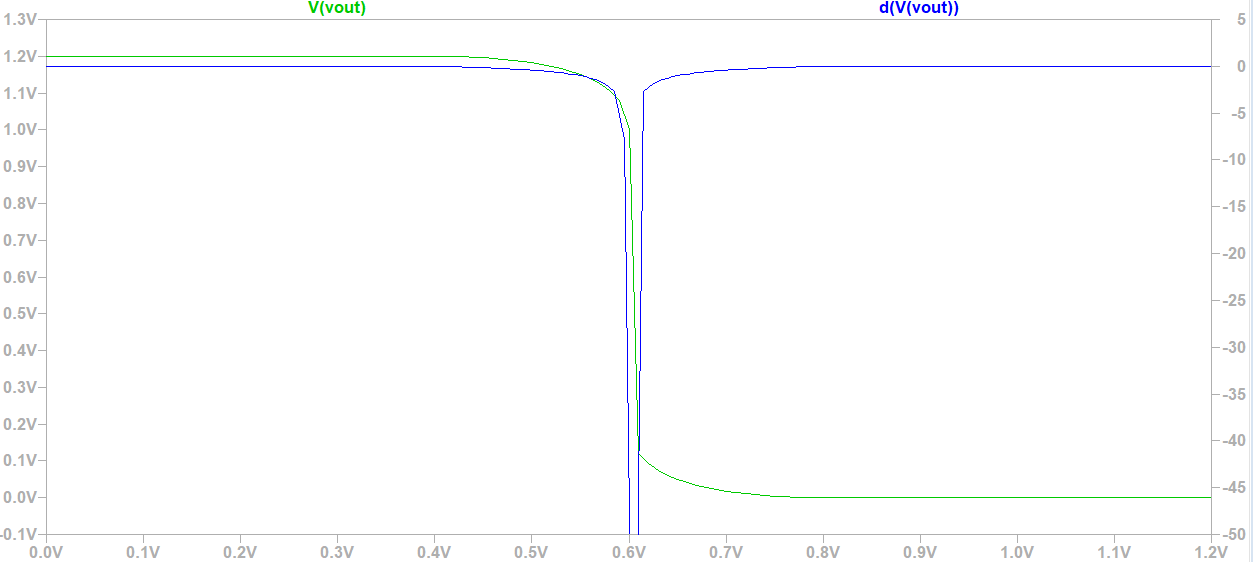
\includegraphics[width=5.5in]{img/p4_8u}
       \caption{RTC Curve for NMOS/PMOS width of \SI{8}{\micro\metre}}
       \label{fig:vtc_8u}
	 \end{figure}
	 
	 To show how the strength of the pull-up network was affected by an increase in the
	 relative widths between the NMOS and the PMOS, the PMOS transistor was given a width
	 of \SI{16}{\micro\metre}.
     
     \begin{figure}[h!]
     	\centering
       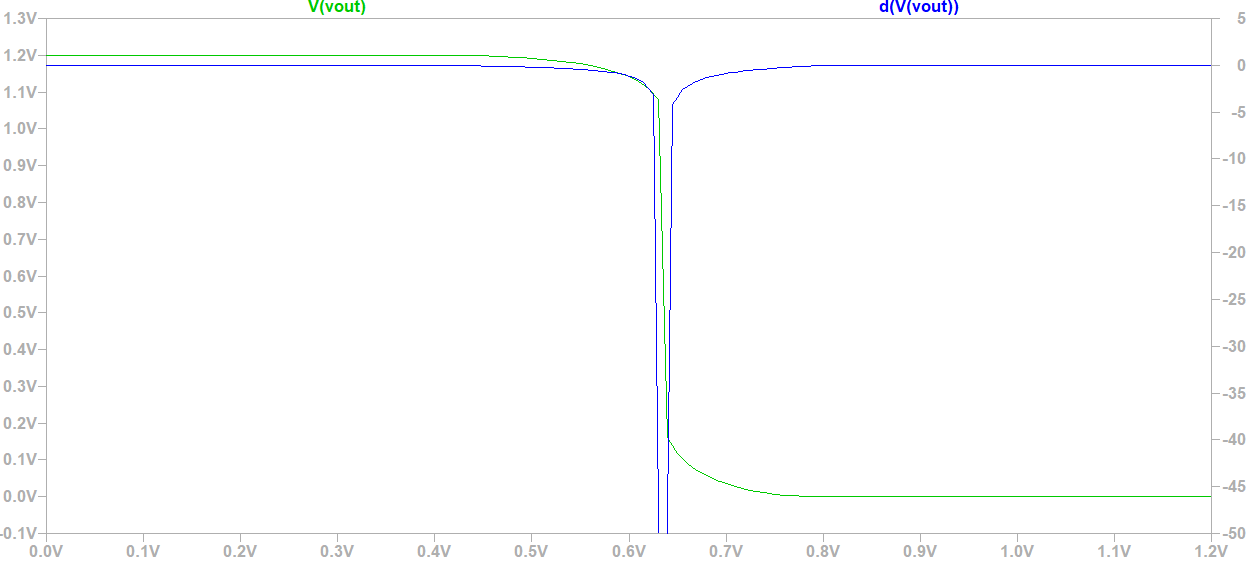
\includegraphics[width=5.5in]{img/p4_16u}
       \caption{RTC Curve for PMOS width of \SI{16}{\micro\metre}}
       \label{fig:vtc_16u}
	 \end{figure}
	 
	 \pagebreak
	
	\begin{table}[h!]
		\renewcommand{\arraystretch}{1.3}
		\setlength{\tabcolsep}{12pt}
		\caption{Simulated parameters of CMOS inverters}
		\begin{center}
		    \begin{tabular}{|c|c|c|c|c|c|c|c|}\hline
		    $W_p$ (\SI{}{\micro\metre}) &
		     $V_{OH}$ & $V_{OL}$ & $V_{IH}$ & $V_{IL}$ & $V_{th}$ & NMH & NML \\\hline
		    8 & 1.2 & 0 & 0.652 & 0.555 & 0.606 & 0.555 & 0.548 \\\hline
		    16 & 1.2 & 0 & 0.691 & 0.597 & 0.636 & 0.597 & 0.509 \\\hline
		    \end{tabular}
		\end{center}
		\label{tab:cmos}
	\end{table}

	Table \ref{tab:cmos} shows the various parameters derived from the
	simulation of both CMOS inverters. The noise margins were also
	calculated to show the tolerance this device would have inside a
	larger network.\\

	The results show that when the relative strength of the pull-up network (PMOS)
	was increased (relative to NMOS), the noise margins on the high end increased
	while they decreased on the low end. This makes sense as signal output will
	remain higher for longer if the PMOS strength is increased. Relatively close noise
	margins were achieved when the $K_r$ ratio was kept at $1$ in the
	$W_p = \SI{8}{\micro\metre}$ case.\\

	Looking back at the prelab calculations, both the $V_{th}$ derived when the $W_p$
	value is doubled ($0.634V$) and the $V_{th}$ value at NML = NMH ($0.6V$) agree
	with the simulated values: $0.636V$ and $0.606V$ respectively.

	\section*{CMOS Inveter (Dynamic)}
	The dynamic behaviour of a CMOS can be interpreted as its VTC curve when
	the output node is under capacitive load. The rise and fall times are defined
	as the time it takes $V_{out}$ to rise and fall from $V_{10\%}$ to $V_{90\%}$.
	
	\pagebreak

	\begin{figure}[h!]
     	\centering
       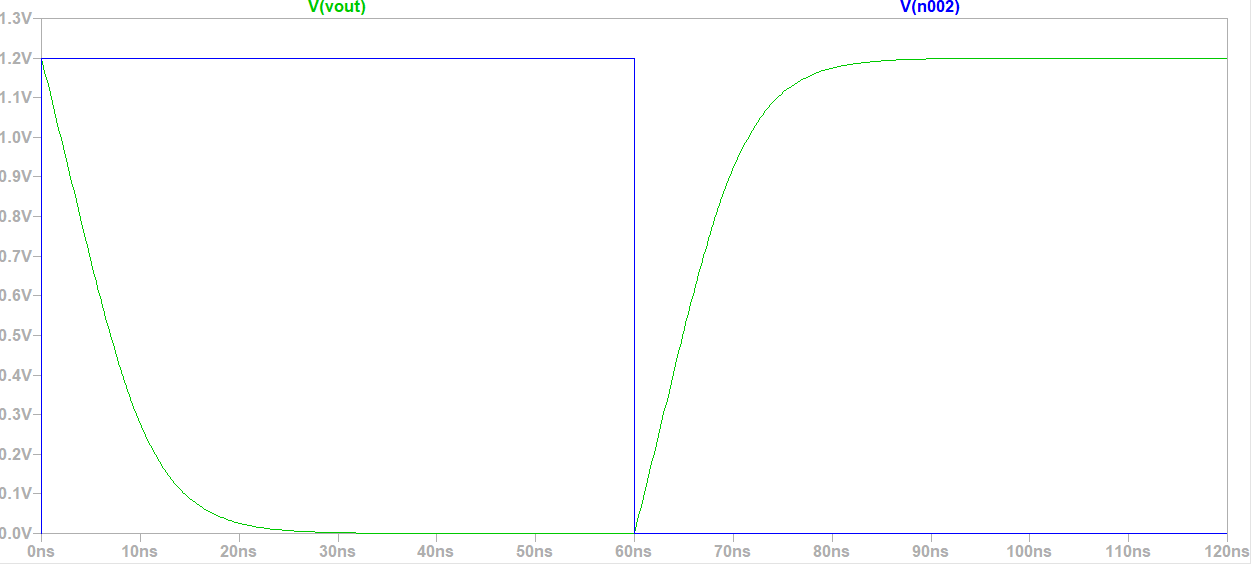
\includegraphics[width=5.5in]{img/p5_8u}
       \caption{Dynamic behaviour of CMOS with $W_p = \SI{8}{\micro\metre}$}
       \label{fig:rs_8u}
	 \end{figure}

	\begin{figure}[h!]
     	\centering
       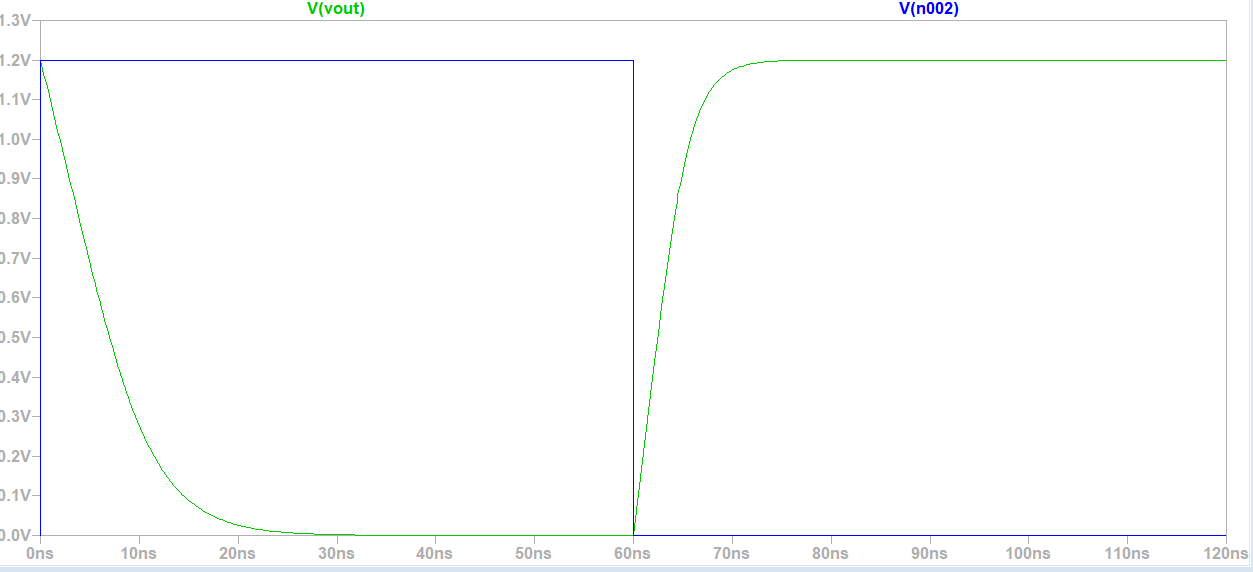
\includegraphics[width=5.5in]{img/p5_16u}
       \caption{Dynamic behaviour of CMOS with $W_p = \SI{16}{\micro\metre}$}
       \label{fig:rs_16u}
	 \end{figure}

	Figures \ref{fig:rs_8u} and \ref{fig:rs_16u} show the inputs and output of the
	CMOS inverter when under a capative load of \SI{25}{\pico\farad}. It can be
	seen that when the PMOS strength is increased, the rise time of the inverter
	will decrease because the PUN strength is able to charge the load faster.


	\begin{table}[h!]
		\renewcommand{\arraystretch}{1.3}
		\setlength{\tabcolsep}{12pt}
		\caption{Rise and Fall times of CMOS inveter under load}
		\begin{center}
		    \begin{tabular}{|c|c|c|}\hline
		    $W_p$ (\SI{}{\micro\metre}
		       & $t_{fall}$ & $t_{rise}$ \\\hline
		    8  & \SI{12.45}{\nano\s} & \SI{12.55}{\nano\s} \\\hline
		    16 & \SI{12.35}{\nano\s} & \SI{6.17}{\nano\s}  \\\hline
		    \end{tabular}
		\end{center}
		\label{tab:p5}
	\end{table}

	Table \ref{tab:p5} shows what was previously described. Then the strength
	of the PMOS was increased, only the rise time was affected by halving it to
	about \SI{6}{\nano\s}.

	\section*{Ring Oscillator}

	Ring oscillation is a special circuit that will exhibit an oscillating
	behaviour. It works by placing a circular chain of an odd number of
	inverters in series such that the signal on nodes between inverters will
	oscillate. The oscillation period is based on the load on the circuit which
	can be simulated with a capacitor between each inverter.

	\begin{figure}[h!]
     	\centering
       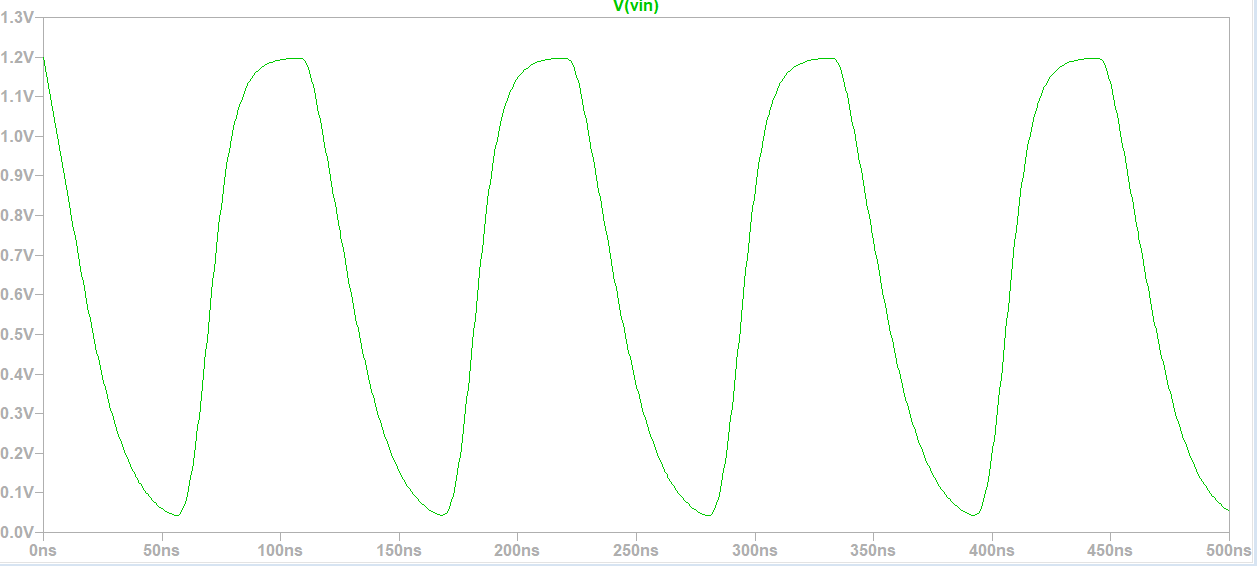
\includegraphics[width=5.5in]{img/p6_no_load}
       \caption{Ring oscillation with only parasitic load}
       \label{fig:os_n}
	 \end{figure}

	\begin{figure}[h!]
     	\centering
       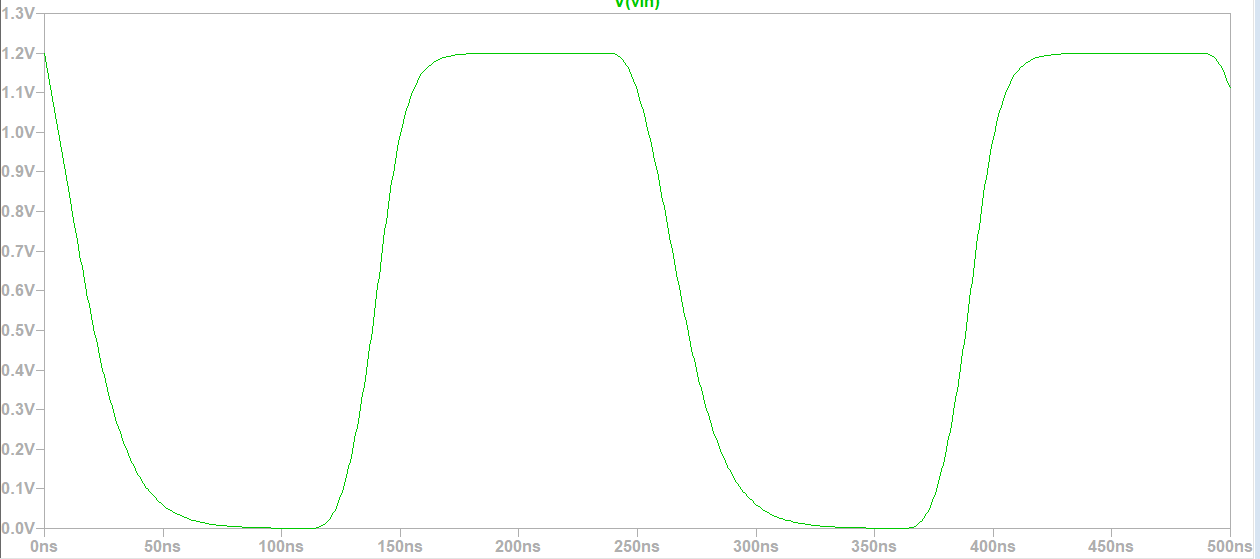
\includegraphics[width=5.5in]{img/p6_load}
       \caption{Ring oscillation with parasitic load and circuit load of \SI{50}{\pico\farad}}
       \label{fig:os_l}
	\end{figure}

	Figures \ref{fig:os_n} and \ref{fig:os_l} show the oscillation periods with and
	without a \SI{50}{\pico\farad} load on each inverter node. The oscillation period
	will increase with the load which is expected because it will take longer to charge
	up a larger capacitor in the loaded case.\\

	Another change that can be made to the ring oscillator is to change $V_{DD}$.
	
	\pagebreak

	\begin{table}[h!]
		\renewcommand{\arraystretch}{1.3}
		\setlength{\tabcolsep}{12pt}
		\caption{Oscillation period when varying $V_{DD}$}
		\begin{center}
		    \begin{tabular}{|c|c|c|}\hline
		    $V_{DD}$ & Period (\SI{}{\nano\s}) & Rise/Fall time per inverter \\\hline
		    1   & \SI{166.95}{\nano\s} & 16.695 \\\hline
		    1.2 & \SI{109.61}{\nano\s} & 10.961 \\\hline
		    2   & \SI{43}{\nano\s} & 4.3 \\\hline
		    \end{tabular}
		\end{center}
		\label{tab:p6}
	\end{table}

	Table \ref{tab:p6} shows the effect that varying $V_{DD}$ has on the period of
	oscillation on the overall ring oscillator. The rise/fall time per inverter is
	found with the assumption that the rise and fall times are about even and that each
	inverter is identical. The period can then be divided by $2N$ where $N$ is the number
	of inverters in the ring. Looking at the results, it makes sense that the period
	should decrease when increasing $V_{DD}$ because the capacitor is driven with more
	current from the inverters when the supply voltage is higher.\\

	Equation \ref{eq:leff}, derived from the prelab, shows the relationship
	between the load, no load, external capacitance to the load capacitance.

	\begin{equation}
	\label{eq:leff}
	C_{Leff} = \frac{t_{noload} \cdot C_{ext}}{t_{load} - t_{noload}}
	\end{equation}
	\begin{equation}
	\label{eq:leff_actual}
	C_{Leff} = \frac{\SI{109.61}{\nano\s} \cdot \SI{50}{\pico\farad}}{\SI{240.30}{\nano\s} - \SI{109.61}{\nano\s}} = \SI{41.90}{\pico\farad}
	\end{equation}

	The experimental value found in Equation \ref{eq:leff_actual} is close the
	to predicated value in the prelab. 

	\section*{Conclusion}
	This exercise looked at the static and dynamic behaviour of CMOS inverters. It
	plotted VTC curves for varying relative powers of the PUN and PDN. The rise and
	fall times were then experimented with by adding a capative load to the output of
	the inverter. PUN strength was increased to show the effect this has on the rise time
	of the inverter. Finally, a ring oscillator was evaluated by running the oscillation
	with and without a load. The ring oscillator was also changed by varying its supply
	voltage to show how higher supplies would charge the loads faster. The goals of
	the this exercise were reached as the circuits were successfully simulated and the
	prelab calculations were supported by the simulation results.

\end{document}
